\documentclass[a4paper, 11pt]{article}
\usepackage{geometry}
\usepackage{graphicx}
\usepackage{tikz}
\usetikzlibrary{automata, positioning, arrows.meta}

% Page layout settings
\geometry{margin=1in}



\begin{document}

\section*{Aufgabe 1 \hspace{0.5em} \normalfont Your Names}

\begin{center}
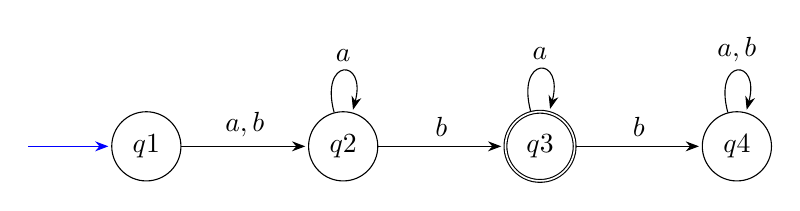
\begin{tikzpicture}[shorten >=1pt, node distance=2.5cm, on grid, auto, >=Stealth]

% Define the states
\node[state] (q1) {$q1$};
\node[state] (q2) [right=of q1] {$q2$};
\node[state, accepting] (q3) [right=of q2] {$q3$};
\node[state] (q4) [right=of q3] {$q4$};

% Initial arrow
\draw[->, color=blue] (-1.5, 0) -- (q1);

% Transitions
\path[->] 
    (q1) edge node {$a, b$} (q2)
    (q2) edge[loop above] node {$a$} ()
         edge node {$b$} (q3)
    (q3) edge[loop above] node {$a$} ()
         edge node {$b$} (q4)
    (q4) edge[loop above] node {$a, b$} ();

\end{tikzpicture}
\end{center}





\vspace{3cm}
\hrule
\end{document}

